\documentclass[12pt]{scrartcl}
\input{../styles/Packages.tex}
\input{../styles/FormatAndHeader.tex}

\setcounter{sheetnr}{4} % Nummer des Übungsblattes
\setcounter{exnum}{1} % Nummer der Aufgabe

% Beginn des eigentlichen Dokuments

\begin{document}

% Aufgabe 1
\exercise{2-3-4-Bäume, Rot-Schwarz-Bäume}
  \begin{enumerate}
    \item Baum T1
      \begin{figure}[!h]
        \centering
        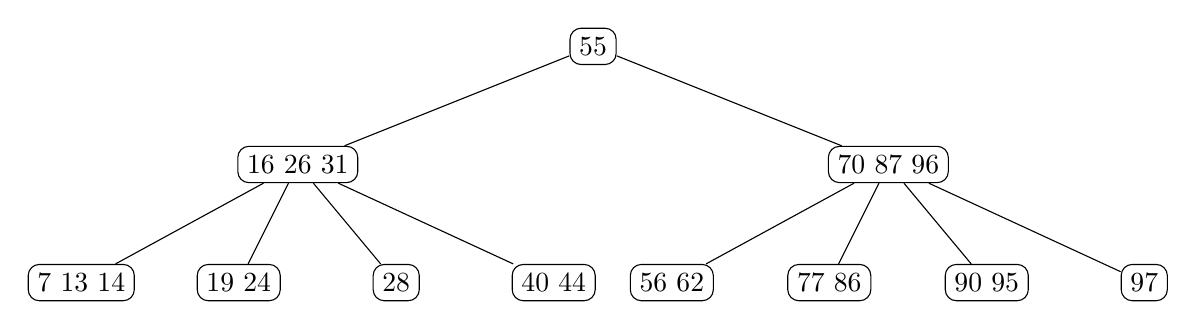
\begin{tikzpicture}
          \node[rectangle,rounded corners,draw] (a) at(0,0) {55}
            child {node [rectangle,rounded corners,draw] (b) at(-3,0) {16 26 31}
              child {node [rectangle,rounded corners,draw] (c) at(-0.5,0) {7 13 14}}
              child {node [rectangle,rounded corners,draw] (d) at(0,0) {19 24}}
              child {node [rectangle,rounded corners,draw] (e) at(0.5,0) {28}}
              child {node [rectangle,rounded corners,draw] (f) at(1,0) {40 44}}
              }
            child {node [rectangle,rounded corners, draw] (g) at(3,0) {70 87 96}
              child {node [rectangle,rounded corners, draw] (h) at(-0.5,0) {56 62}}
              child {node [rectangle,rounded corners, draw] (i) at(0,0) {77 86}}
              child {node [rectangle,rounded corners, draw] (j) at(0.5,0) {90 95}}
              child {node [rectangle,rounded corners, draw] (j) at(1,0) {97}}
            };
        \end{tikzpicture}
        \caption{96 nach oben ziehen, dann 90 einfügen}
        \label{fig:baum}
      \end{figure}

      \begin{figure}[!h]
        \centering
        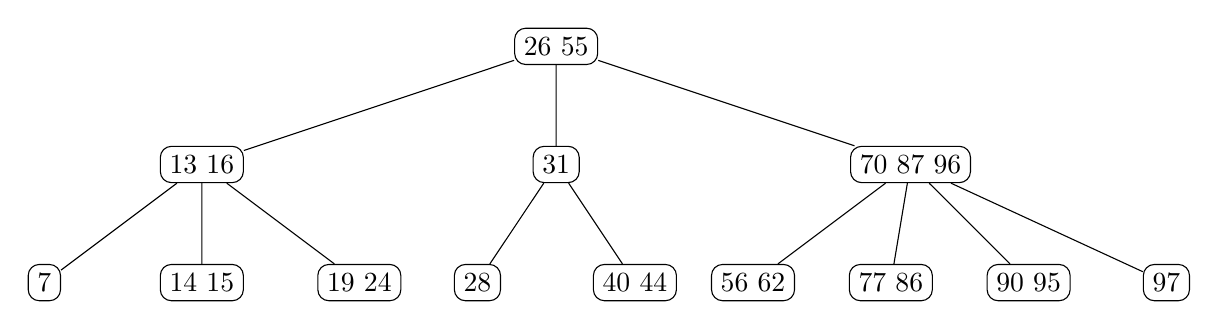
\begin{tikzpicture}
          \node[rectangle,rounded corners,draw] (a) at(0,0) {26 55}
            child {node [rectangle,rounded corners,draw] (b) at(-3,0) {13 16}
              child {node [rectangle,rounded corners,draw] (c) at(-0.5,0) {7}}
              child {node [rectangle,rounded corners,draw] (d) at(0,0) {14 15}}
              child {node [rectangle,rounded corners,draw] (e) at(0.5,0) {19 24}}
              }
            child {node [rectangle,rounded corners,draw] (f) at(0,0) {31}
              child {node [rectangle,rounded corners,draw] (g) at(-0.25,0) {28}}
              child {node [rectangle,rounded corners,draw] (h) at(0.25,0) {40 44}}
              }
            child {node [rectangle,rounded corners, draw] (i) at(3,0) {70 87 96}
              child {node [rectangle,rounded corners, draw] (j) at(0.25,0) {56 62}}
              child {node [rectangle,rounded corners, draw] (k) at(0.5,0) {77 86}}
              child {node [rectangle,rounded corners, draw] (l) at(0.75,0) {90 95}}
              child {node [rectangle,rounded corners, draw] (m) at(1,0) {97}}
            };
        \end{tikzpicture}
        \caption{13 und 26 nach oben ziehen, dann 15 einfügen}
        \label{fig:baum}
      \end{figure}

    \item Rot-Schwarz-Baum
      \begin{figure}[!h]
        \centering
        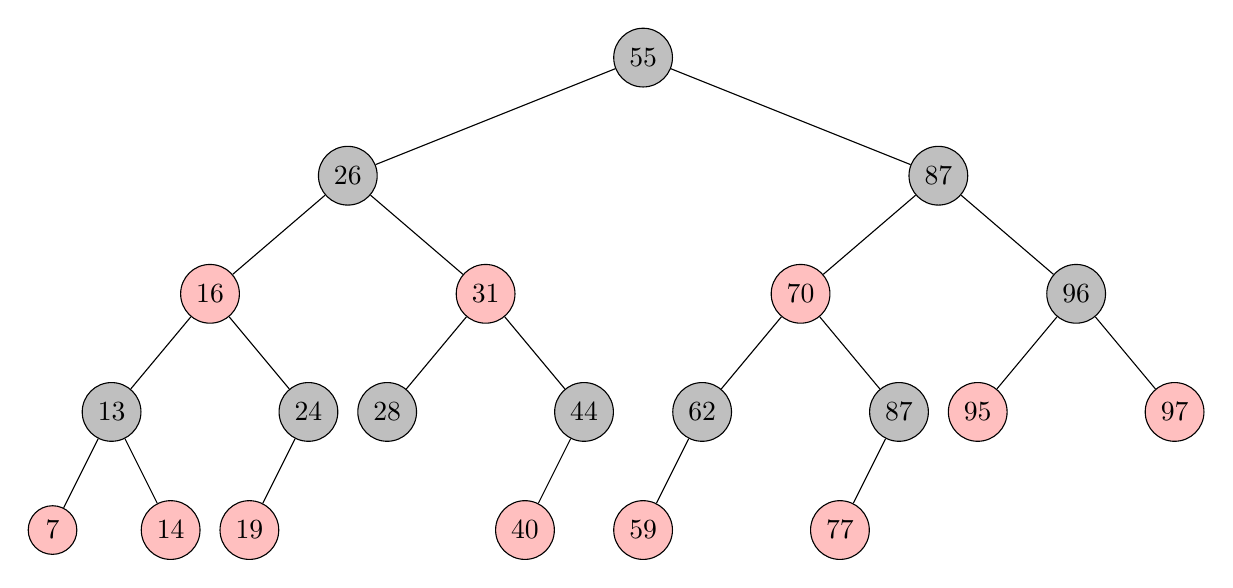
\begin{tikzpicture}
          \node[circle,fill=lightgray,draw] (a) {55} 
            child {node [circle,fill=lightgray,draw] (b) at(-3,0) {26}
              child {node [circle,fill=pink,draw] (c) at(-1,0) {16}
                child {node[circle,fill=lightgray,draw] (d) at(-0.5,0){13}
                  child {node[circle,fill=pink,draw] (e) {7}}
                  child {node[circle,fill=pink,draw] (f) {14}}
                }
                child {node[circle,fill=lightgray,draw] (g) at(0.5,0) {24}
                  child {node[circle,fill=pink,draw] (h) {19}}
                  child[missing]{node{}} 
                }
              }
             child {node [circle,fill=pink,draw] (i) at(1,0) {31}
                child {node[circle,fill=lightgray,draw] (j) at(-0.5,0) {28}}
                child {node[circle,fill=lightgray,draw] (k) at(0.5,0) {44}
                  child {node[circle,fill=pink,draw] (l) {40}}
                  child[missing]{node{}}
                  }
                }
              }
            child {node [circle,fill=lightgray,draw] (m) at(3,0) {87}
              child {node [circle,fill=pink,draw] (n) at(-1,0) {70}
                child {node [circle,fill=lightgray,draw] (o) at(-0.5,0) {62}
                  child {node [circle,fill=pink,draw] (p) {59}}
                  child[missing]{node{}}
                  }
                child {node [circle,fill=lightgray,draw] (q) at(0.5,0) {87}
                  child {node [circle,fill=pink,draw] (r) {77}}
                  child[missing]{node{}}
                  }
                }
              child {node [circle,fill=lightgray,draw] (s) at(1,0) {96}
                child {node [circle,fill=pink,draw] (t) at(-0.5,0) {95}}
                child {node [circle,fill=pink,draw] (u) at(0.5,0) {97}}
                }
              };
        \end{tikzpicture}
        \caption{Rot-Schwarz-Baum umwandelt von Baum T1}
        \label{fig:baum}
      \end{figure}

\newpage

     \item Baum T2
      \begin{figure}[!h]
        \centering
        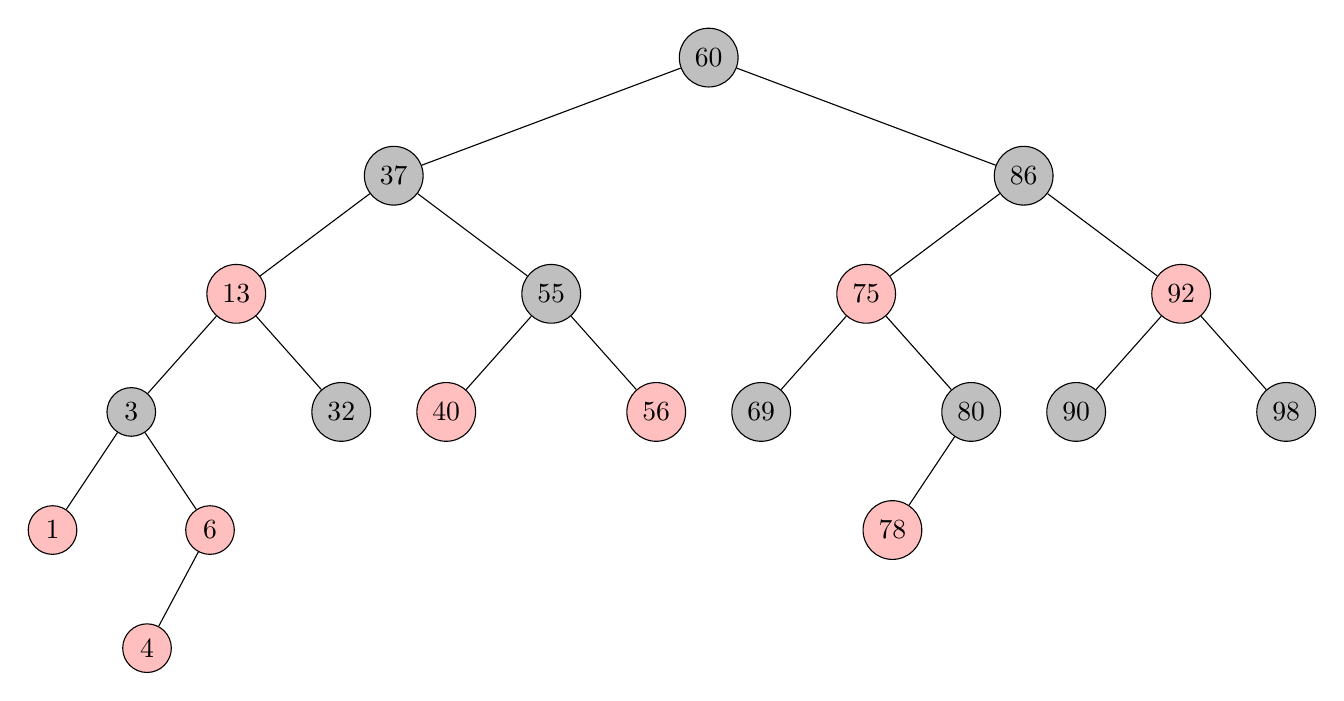
\begin{tikzpicture}
          \node[circle,fill=lightgray,draw] (a) {60} [level/.style ={sibling distance=80mm/#1}]
            child {node [circle,fill=lightgray,draw] (b) {37}
              child {node [circle,fill=pink,draw] (c) {13}
                child {node[circle,fill=lightgray,draw] (d) {3}
                  child {node[circle,fill=pink,draw] (e) {1}}
                  child {node[circle,fill=pink,draw] (f) {6}
                    child {node[circle,fill=pink,draw] (s) {4}}
                    child[missing]{node{}}
                    }
                }
                child {node[circle,fill=lightgray,draw] (g) {32}}
              }
             child {node [circle,fill=lightgray,draw] (h) {55}
                child {node[circle,fill=pink,draw] (i) {40}}
                child {node[circle,fill=pink,draw] (j) {56}}
                }
              }
            child {node [circle,fill=lightgray,draw] (k) {86}
              child {node [circle,fill=pink,draw] (l) {75}
                child {node [circle,fill=lightgray,draw] (m) {69}}
                child {node [circle,fill=lightgray,draw] (n) {80}
                  child {node [circle,fill=pink,draw] (o) {78}}
                  child[missing]{node{}}
                  }
                }
                child {node [circle,fill=pink,draw] (p) {92}
                  child {node [circle,fill=lightgray,draw] (q) {90}}
                  child {node [circle,fill=lightgray,draw] (r) {98}}
                  }
                };
        \end{tikzpicture}
        \caption{4 an den Rot-Schwarz-Baum T2 einfügen}
        \label{fig:baum}
      \end{figure}

      \begin{figure}[!h]
        \centering
        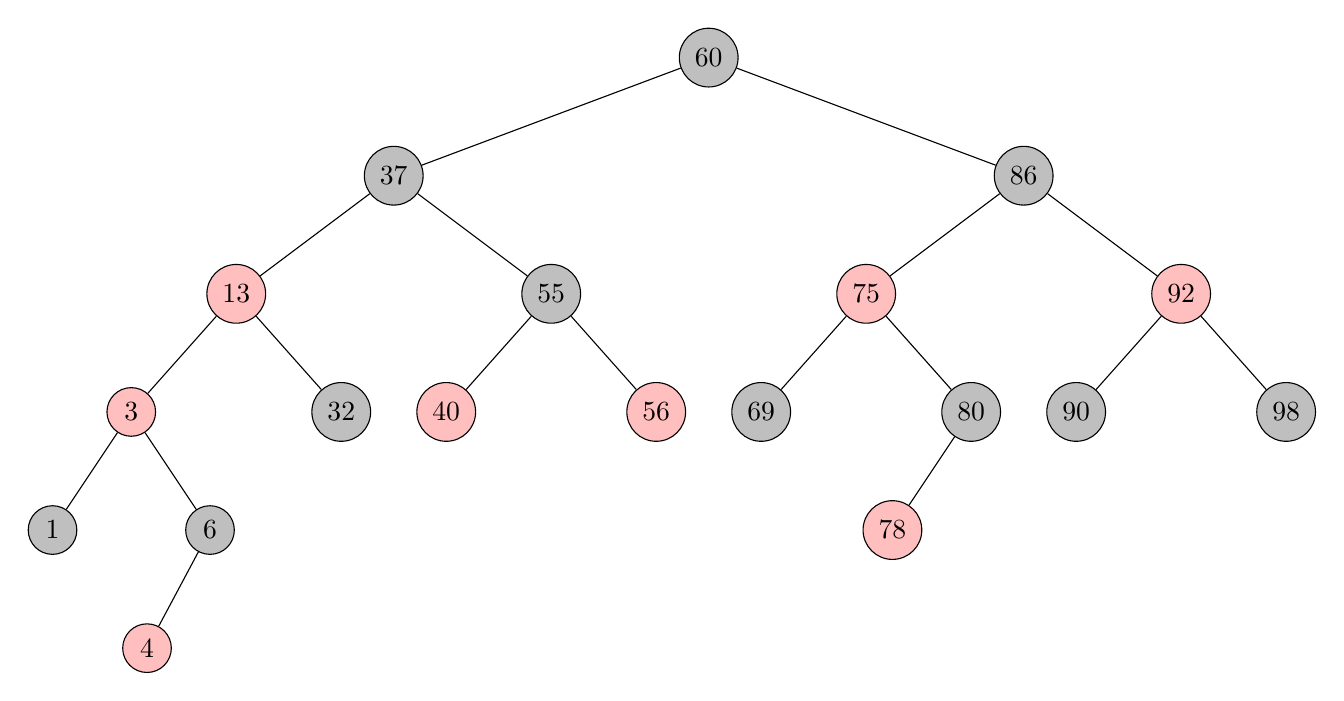
\begin{tikzpicture}
          \node[circle,fill=lightgray,draw] (a) {60} [level/.style ={sibling distance=80mm/#1}]
            child {node [circle,fill=lightgray,draw] (b) {37}
              child {node [circle,fill=pink,draw] (c) {13}
                child {node[circle,fill=pink,draw] (d) {3}
                  child {node[circle,fill=lightgray,draw] (e) {1}}
                  child {node[circle,fill=lightgray,draw] (f) {6}
                    child {node[circle,fill=pink,draw] (s) {4}}
                    child[missing]{node{}}
                    }
                }
                child {node[circle,fill=lightgray,draw] (g) {32}}
              }
             child {node [circle,fill=lightgray,draw] (h) {55}
                child {node[circle,fill=pink,draw] (i) {40}}
                child {node[circle,fill=pink,draw] (j) {56}}
                }
              }
            child {node [circle,fill=lightgray,draw] (k) {86}
              child {node [circle,fill=pink,draw] (l) {75}
                child {node [circle,fill=lightgray,draw] (m) {69}}
                child {node [circle,fill=lightgray,draw] (n) {80}
                  child {node [circle,fill=pink,draw] (o) {78}}
                  child[missing]{node{}}
                  }
                }
                child {node [circle,fill=pink,draw] (p) {92}
                  child {node [circle,fill=lightgray,draw] (q) {90}}
                  child {node [circle,fill=lightgray,draw] (r) {98}}
                  }
                };
        \end{tikzpicture}
        \caption{Rot-Schwarz-Baum T2 umfärben}
        \label{fig:baum}
      \end{figure}

      \begin{figure}[!h]
        \centering
        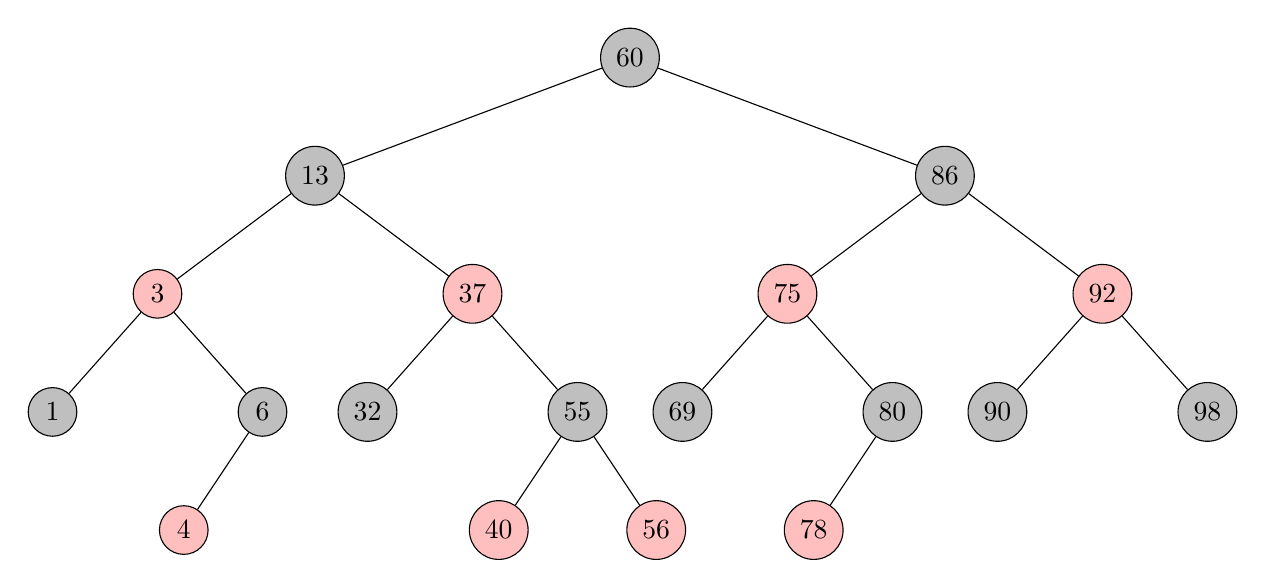
\begin{tikzpicture}
          \node[circle,fill=lightgray,draw] (a) {60} [level/.style ={sibling distance=80mm/#1}]
            child {node [circle,fill=lightgray,draw] (b) {13}
              child {node [circle,fill=pink,draw] (c) {3}
                child {node[circle,fill=lightgray,draw] (d) {1}}
                child {node[circle,fill=lightgray,draw] (e) {6}
                  child {node[circle,fill=pink,draw] (s) {4}}
                  child[missing]{node{}}
                  }
                }
              child {node [circle,fill=pink,draw] (f) {37}
                child {node[circle,fill=lightgray,draw] (g) {32}}
                child {node [circle,fill=lightgray,draw] (h) {55}
                  child {node[circle,fill=pink,draw] (i) {40}}
                  child {node[circle,fill=pink,draw] (j) {56}}
                  }
                }
              }
            child {node [circle,fill=lightgray,draw] (k) {86}
              child {node [circle,fill=pink,draw] (l) {75}
                child {node [circle,fill=lightgray,draw] (m) {69}}
                child {node [circle,fill=lightgray,draw] (n) {80}
                  child {node [circle,fill=pink,draw] (o) {78}}
                  child[missing]{node{}}
                  }
                }
                child {node [circle,fill=pink,draw] (p) {92}
                  child {node [circle,fill=lightgray,draw] (q) {90}}
                  child {node [circle,fill=lightgray,draw] (r) {98}}
                  }
                };
        \end{tikzpicture}
        \caption{Rot-Schwarz-Baum T2 Rotation}
        \label{fig:baum}
      \end{figure}
\end{enumerate}

\newpage

\setcounter{exnum}{4} % Nummer der Aufgabe
\exercise{B-Bäume}

\begin{figure}[!h]
  \centering
  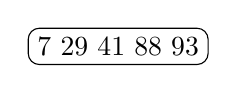
\begin{tikzpicture}
    \node[rectangle,rounded corners,draw] (a) {7 29 41 88 93};
  \end{tikzpicture}
\end{figure}

\begin{figure}[!h]
  \centering
  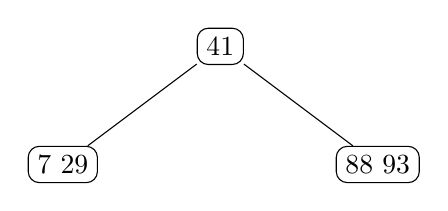
\begin{tikzpicture}
    \node[rectangle,rounded corners,draw] (a) {41}[level/.style ={sibling distance=40mm/#1}]
      child {node [rectangle,rounded corners,draw] (b) {7 29}}
      child {node [rectangle,rounded corners,draw] (c) {88 93}};
  \end{tikzpicture}
  \caption{erste Split}
\end{figure}

\begin{figure}[!h]
  \centering
  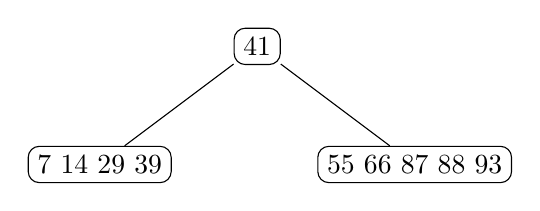
\begin{tikzpicture}
    \node[rectangle,rounded corners,draw] (a) {41}[level/.style ={sibling distance=40mm/#1}]
      child {node [rectangle,rounded corners,draw] (b) {7 14 29 39}}
      child {node [rectangle,rounded corners,draw] (c) {55 66 87 88 93}};
  \end{tikzpicture}
\end{figure}

\begin{figure}[!h]
  \centering
  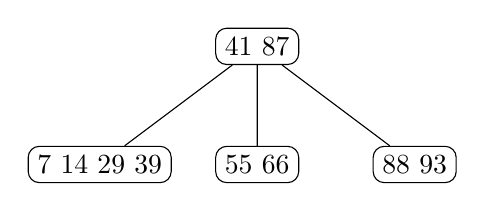
\begin{tikzpicture}
    \node[rectangle,rounded corners,draw] (a) {41 87}[level/.style ={sibling distance=20mm/#1}]
      child {node [rectangle,rounded corners,draw] (b) {7 14 29 39}}
      child {node [rectangle,rounded corners,draw] (c) {55 66}}
      child {node [rectangle,rounded corners,draw] (d) {88 93}};
  \end{tikzpicture}
  \caption{zweites Split}
\end{figure}

\begin{figure}[!h]
  \centering
  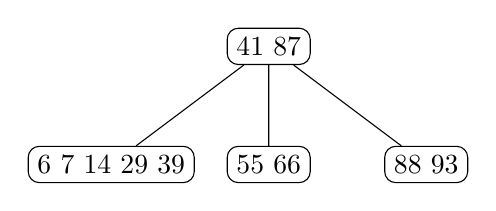
\begin{tikzpicture}
    \node[rectangle,rounded corners,draw] (a) {41 87}[level/.style ={sibling distance=20mm/#1}]
      child {node [rectangle,rounded corners,draw] (b) {6 7 14 29 39}}
      child {node [rectangle,rounded corners,draw] (c) {55 66}}
      child {node [rectangle,rounded corners,draw] (d) {88 93}};
  \end{tikzpicture}
\end{figure}

\begin{figure}[!h]
  \centering
  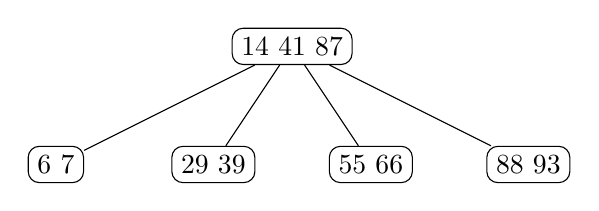
\begin{tikzpicture}
    \node[rectangle,rounded corners,draw] (a) {14 41 87}[level/.style ={sibling distance=20mm/#1}]
      child {node [rectangle,rounded corners,draw] (b) {6 7}}
      child {node [rectangle,rounded corners,draw] (c) {29 39}}
      child {node [rectangle,rounded corners,draw] (d) {55 66}}
      child {node [rectangle,rounded corners,draw] (e) {88 93}};
  \end{tikzpicture}
  \caption{drittes Split}
\end{figure}

\begin{figure}[!h]
  \centering
  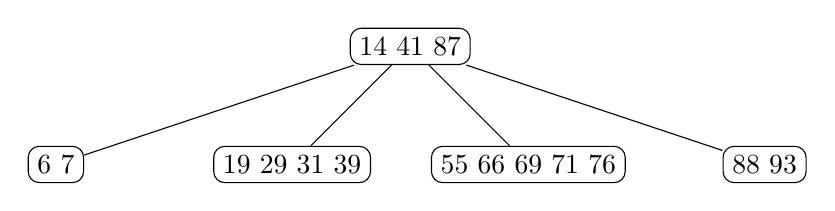
\begin{tikzpicture}
    \node[rectangle,rounded corners,draw] (a) {14 41 87}[level/.style ={sibling distance=30mm/#1}]
      child {node [rectangle,rounded corners,draw] (b) {6 7}}
      child {node [rectangle,rounded corners,draw] (c) {19 29 31 39}}
      child {node [rectangle,rounded corners,draw] (d) {55 66 69 71 76}}
      child {node [rectangle,rounded corners,draw] (e) {88 93}};
  \end{tikzpicture}
\end{figure}

\begin{figure}[!h]
  \centering
  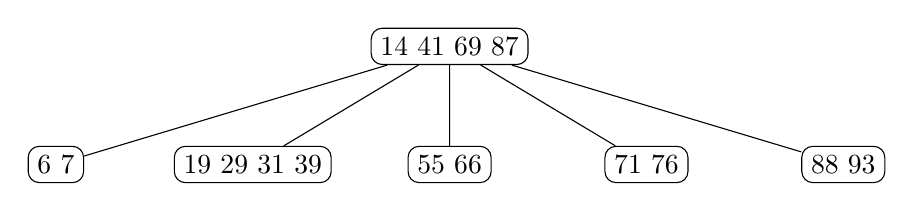
\begin{tikzpicture}
    \node[rectangle,rounded corners,draw] (a) {14 41 69 87}[level/.style ={sibling distance=25mm/#1}]
      child {node [rectangle,rounded corners,draw] (b) {6 7}}
      child {node [rectangle,rounded corners,draw] (c) {19 29 31 39}}
      child {node [rectangle,rounded corners,draw] (d) {55 66}}
      child {node [rectangle,rounded corners,draw] (d) {71 76}}
      child {node [rectangle,rounded corners,draw] (e) {88 93}};
  \end{tikzpicture}
  \caption{viertes Split}
\end{figure}

\begin{figure}[!h]
  \centering
  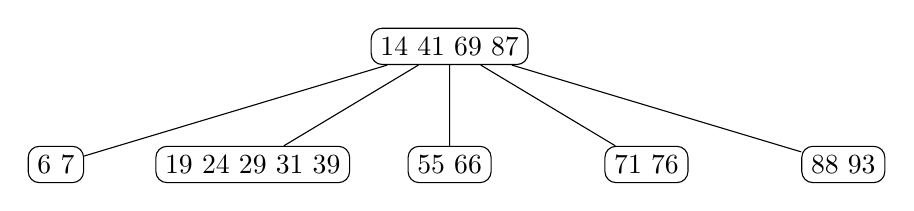
\begin{tikzpicture}
    \node[rectangle,rounded corners,draw] (a) {14 41 69 87}[level/.style ={sibling distance=25mm/#1}]
      child {node [rectangle,rounded corners,draw] (b) {6 7}}
      child {node [rectangle,rounded corners,draw] (c) {19 24 29 31 39}}
      child {node [rectangle,rounded corners,draw] (d) {55 66}}
      child {node [rectangle,rounded corners,draw] (d) {71 76}}
      child {node [rectangle,rounded corners,draw] (e) {88 93}};
  \end{tikzpicture}
\end{figure}

\begin{figure}[!h]
  \centering
  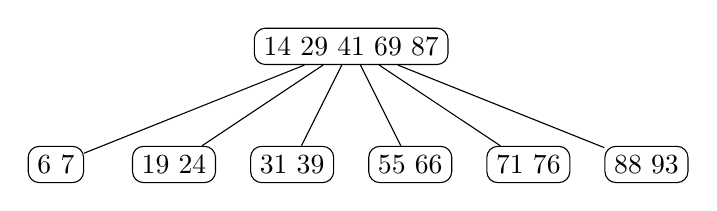
\begin{tikzpicture}
    \node[rectangle,rounded corners,draw] (a) {14 29 41 69 87}
      child {node [rectangle,rounded corners,draw] (b) {6 7}}
      child {node [rectangle,rounded corners,draw] (c) {19 24}}
      child {node [rectangle,rounded corners,draw] (c) {31 39}}
      child {node [rectangle,rounded corners,draw] (d) {55 66}}
      child {node [rectangle,rounded corners,draw] (e) {71 76}}
      child {node [rectangle,rounded corners,draw] (f) {88 93}};
  \end{tikzpicture}
  \caption{fünftes Split}
\end{figure}

\newpage

\begin{figure}[!h]
  \centering
  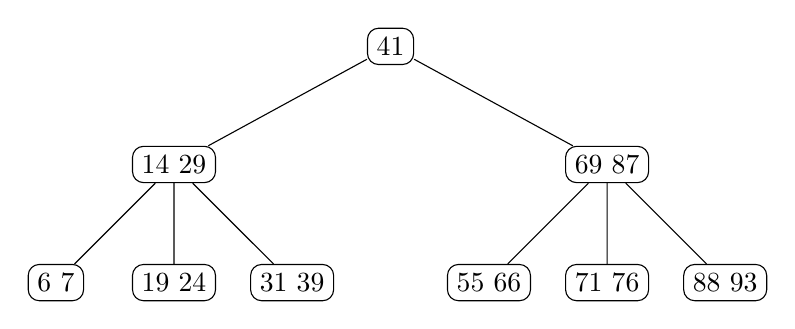
\begin{tikzpicture}
    \node[rectangle,rounded corners,draw] (a) {41}
      child {node [rectangle,rounded corners,draw] (b) at(-2,0) {14 29}
        child {node [rectangle,rounded corners,draw] (c) {6 7}}
        child {node [rectangle,rounded corners,draw] (d) {19 24}}
        child {node [rectangle,rounded corners,draw] (e) {31 39}}
        }
      child {node [rectangle,rounded corners,draw] (f) at(2,0) {69 87}
        child {node [rectangle,rounded corners,draw] (g) {55 66}}
        child {node [rectangle,rounded corners,draw] (h) {71 76}}
        child {node [rectangle,rounded corners,draw] (i) {88 93}}
        };
  \end{tikzpicture}
  \caption{sechtes Split}
\end{figure}

\end{document}